\documentclass[10pt]{article}
\usepackage{amsmath,amsfonts,times}
\usepackage{graphicx,color,tikz,pgfplots}
\usepackage[paperwidth=4.8cm,paperheight=4.6cm,lmargin=0in,rmargin=0in,tmargin=0.in,bmargin=0.in]{geometry}
\usepackage{bm}
\usetikzlibrary{arrows,shadings,shapes.arrows,decorations.pathreplacing,calc, positioning}
\usepgfplotslibrary{fillbetween}

\pgfplotsset{
  compat=newest
}

\newlength{\dx}
\setlength{\dx}{1.5cm}

\newlength{\dy}
\setlength{\dy}{1.cm}

\newlength{\circleRadius}
\setlength{\circleRadius}{0.95\dx}

\definecolor{outside}{rgb}{0, 1, 0}
\definecolor{cutcell}{rgb}{0, 0.5, 1}
\definecolor{inside}{rgb}{1, 0, 0}

\tikzset{
  edge/.style={thick, draw=black},
  normal/.style={very thick, draw=black, ->},
  vertex/.style={circle, inner sep=0pt, minimum width=4pt, draw=black, fill=black, node contents={}},
}

\begin{document}
\centering
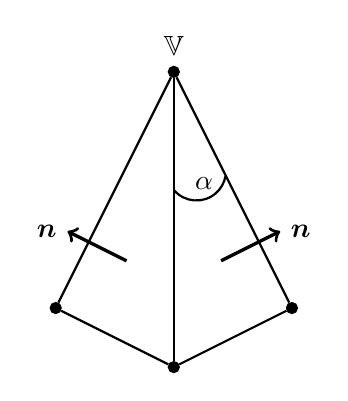
\begin{tikzpicture}

  
  \node (v0) at (0,0) [vertex];
  \node (v1) at (-\dx, -2\dx) [vertex];
  \node (v2) at (\dx,-2\dx) [vertex];
  \node (v3) at (0,-2.5\dx) [vertex];

  \draw[edge] (v0) -- (v1) -- (v3) -- (v2) -- (v0);
  \draw[edge] (v0) -- (v3);

  \draw[normal] (-0.4\dx, -1.6\dx) --++(-0.5\dx, 0.25\dx) node[above, left] {$\bm{n}$};
  \draw[normal] (0.4\dx, -1.6\dx) --++(0.5\dx, 0.25\dx) node[above, right] {$\bm{n}$};
  \node[anchor=south] at (v0.north) {$\mathbb{V}$};

  \draw[thick] (0, -\dx) arc (220:350:0.25\dx) node [midway, above] {$\alpha$};
  
\end{tikzpicture}

\end{document} 
